\section{Data source}
The data source for this study are listed below, which is also available at this \href{https://drive.google.com/drive/folders/1nVRsTTLyp0k4gV46zZ6d8C2gQEJnXjfd?usp=sharing}{link}. For a quick overview, Figure \ref{confirm} shows the daily confirmed COVID-19 cases/deaths and Google (residential) mobility trends of Singapore from February 17th 2020 to Oct 29th 2021.
\begin{itemize}
	\item COVID-19 cases/deaths/vaccines: The COVID-19 related data comes from \href{https://data.world/hxchua/covid-19-singapore}{data.world}. We choose several data points and verify it with \href{https://www.moh.gov.sg/covid-19/past-updates}{official MOH report}. For the missing vaccine data (from Jan 11th 2021 to June 30th 2021), we fill it with data from \href{https://ourworldindata.org/covid-vaccinations?country=SGP}{Our World in Data} and perform linear interpolation to make it continuous.
	\item Epidemiology: The epidemiology data of COVID-19, such as duration parameters (for example, duration between exposed state and infectious state), age-linked disease probability (for example, relative susceptibility to infection), is built in the library \href{https://github.com/InstituteforDiseaseModeling/covasim}{covasim}. 
	\item Demographics: The population age distribution data comes from this \href{https://github.com/neherlab/covid19_scenarios/blob/master/src/assets/data/ageDistribution.json}{Github repo} and is built in the library \href{https://github.com/InstituteforDiseaseModeling/covasim}{covasim}. However, because the Department of Statistics of Singapore only releases the resident population age distribution, we are not able to verify the correctness of this data.
	\item Mobility: We use \href{https://www.google.com/covid19/mobility/}{Google Community Mobility Reports} as the indicator of mobility. The reports provide the changes in movement trends across different categories of activities, which includes residential, retail and recreation, groceries and pharmacies, parks, transit stations, and workplaces. We collect this data from \href{https://ourworldindata.org/covid-google-mobility-trends}{Our World in Data}.
	\item Policy: We use \href{https://github.com/OxCGRT/covid-policy-tracker/tree/master/data}{mask policy indicator}, which is categorized into five categories: 0 - no policy; 1 - recommended; 2 - required in specified public spaces; 3 - required in all public spaces; 4 - required outside the home at all times. We also collect other relevant policy data (such as quarantine policy, face covering policy) from \href{https://www.moh.gov.sg/covid-19/past-updates}{official MOH report}.
\end{itemize}
\begin{figure}[htbp]
	\centering
	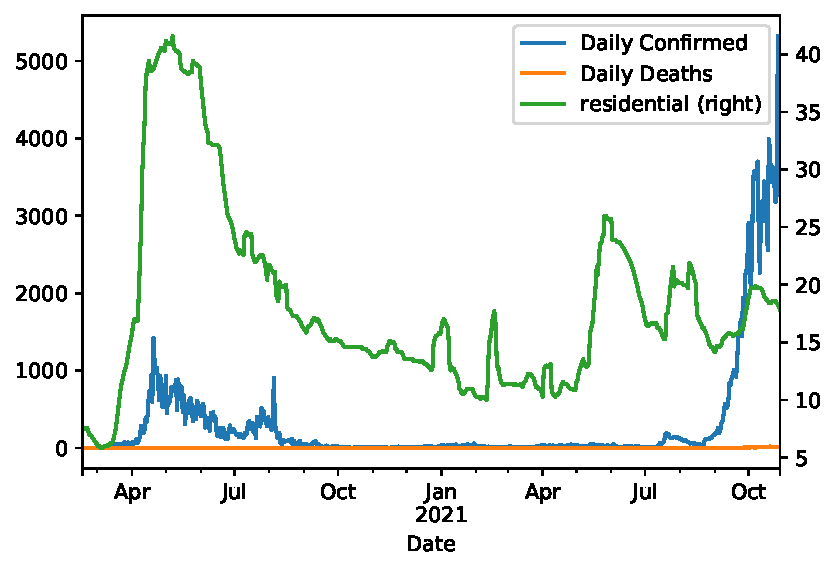
\includegraphics[width=0.9\linewidth]{data/confirmed.pdf}
	\caption{Daily COVID-19 counts and Google mobility trends}
	\label{confirm}
\end{figure}